\renewcommand{\thefigure}{\theenumi}
\renewcommand{\thetable}{\theenumi}
%%
\begin{enumerate}[label=\thesection.\arabic*
,ref=\thesection.\theenumi]

%
\item
Generate $10^6$ samples of the random variable
%
\begin{equation}
X = \sum_{i=1}^{12}U_i -6
\end{equation}
%
using a C program, where $U_i, i = 1,2,\dots, 12$ are  a set of independent uniform random variables between 0 and 1
and save in a file called gau.dat

%
\item
Load gau.dat in python and plot the empirical CDF of $X$ using the samples in gau.dat. What properties does a CDF have?
\\
\solution The CDF of $X$ is plotted in Fig. \ref{fig:gauss_cdf}
\begin{figure}
\centering
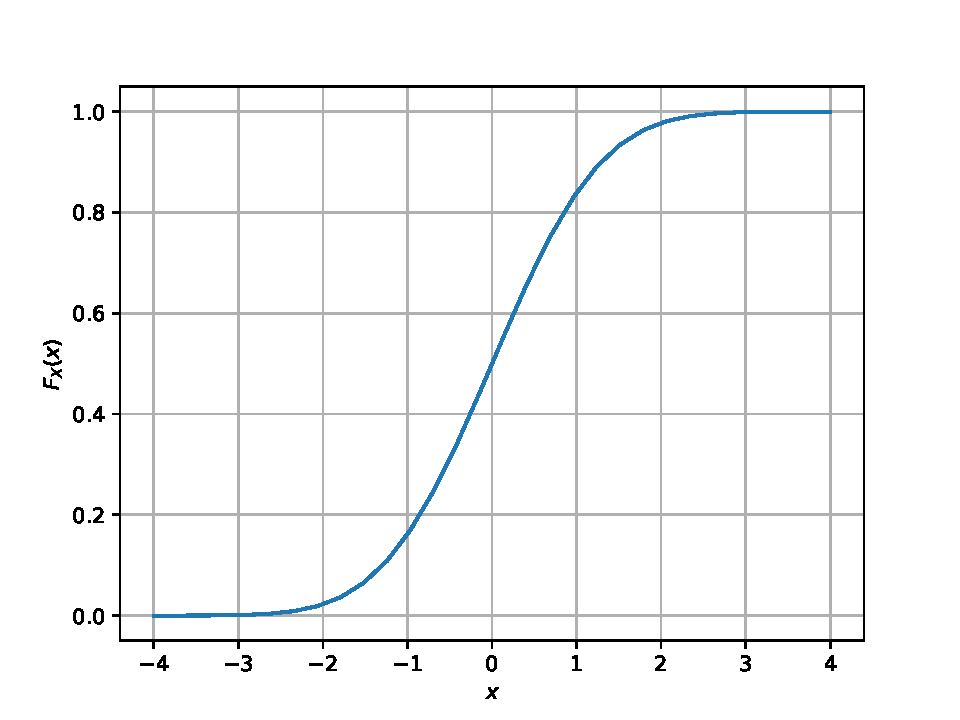
\includegraphics[width=\columnwidth]{./figs/clt/gauss_cdf}
\caption{The CDF of $X$}
\label{fig:gauss_cdf}
\end{figure}
\item
Load gau.dat in python and plot the empirical PDF of $X$ using the samples in gau.dat. The PDF of $X$ is defined as
\begin{align}
p_{X}(x) = \frac{d}{dx}F_{X}(x)
\end{align}
What properties does the PDF have?
\\
\solution The PDF of $X$ is plotted in Fig. \ref{fig:gauss_pdf} using the code below
\begin{lstlisting}
codes/clt/pdf_plot.py
\end{lstlisting}

\begin{figure}
\centering
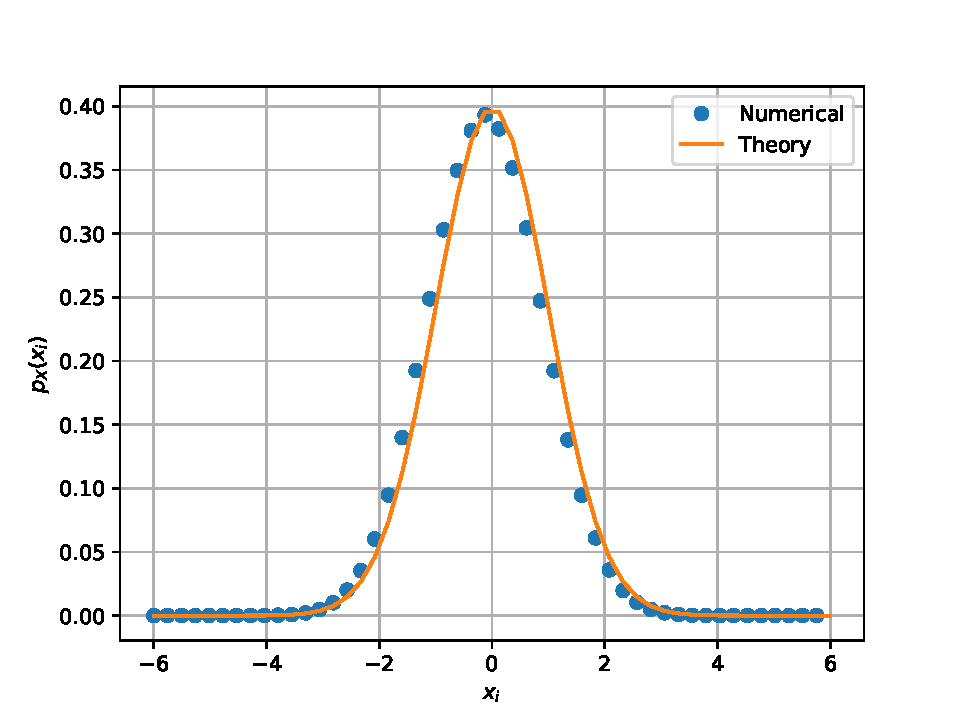
\includegraphics[width=\columnwidth]{./figs/clt/gauss_pdf}
\caption{The PDF of $X$}
\label{fig:gauss_pdf}
\end{figure}

\item Find the mean and variance of $X$ by writing a C program.
\item Given that 
\begin{align}
p_{X}(x) = \frac{1}{\sqrt{2\pi}}\exp\brak{-\frac{x^2}{2}}, -\infty < x < \infty,
\end{align}
repeat the above exercise theoretically.
%
\end{enumerate}



